\label{chap:testing}
\section{PolyBench}
The framework is tested with polyBench 1.0\footnote{\url{http://www-roc.inria.fr/~pouchet/software/polybench/}}
and the results are shown in the next section. PolyBench is a set of computationally intensive programs often
used in the polyhedral community. There are benchmarks from linear algebra, datamining, stencil computation
and solver and manipulation algorithms operating on matrices. On those benchmarks Polly extracts the relevant SCoPs and optimizes them automatically.

\section{Experimental results}
\begin{figure}
\begin{center}
  %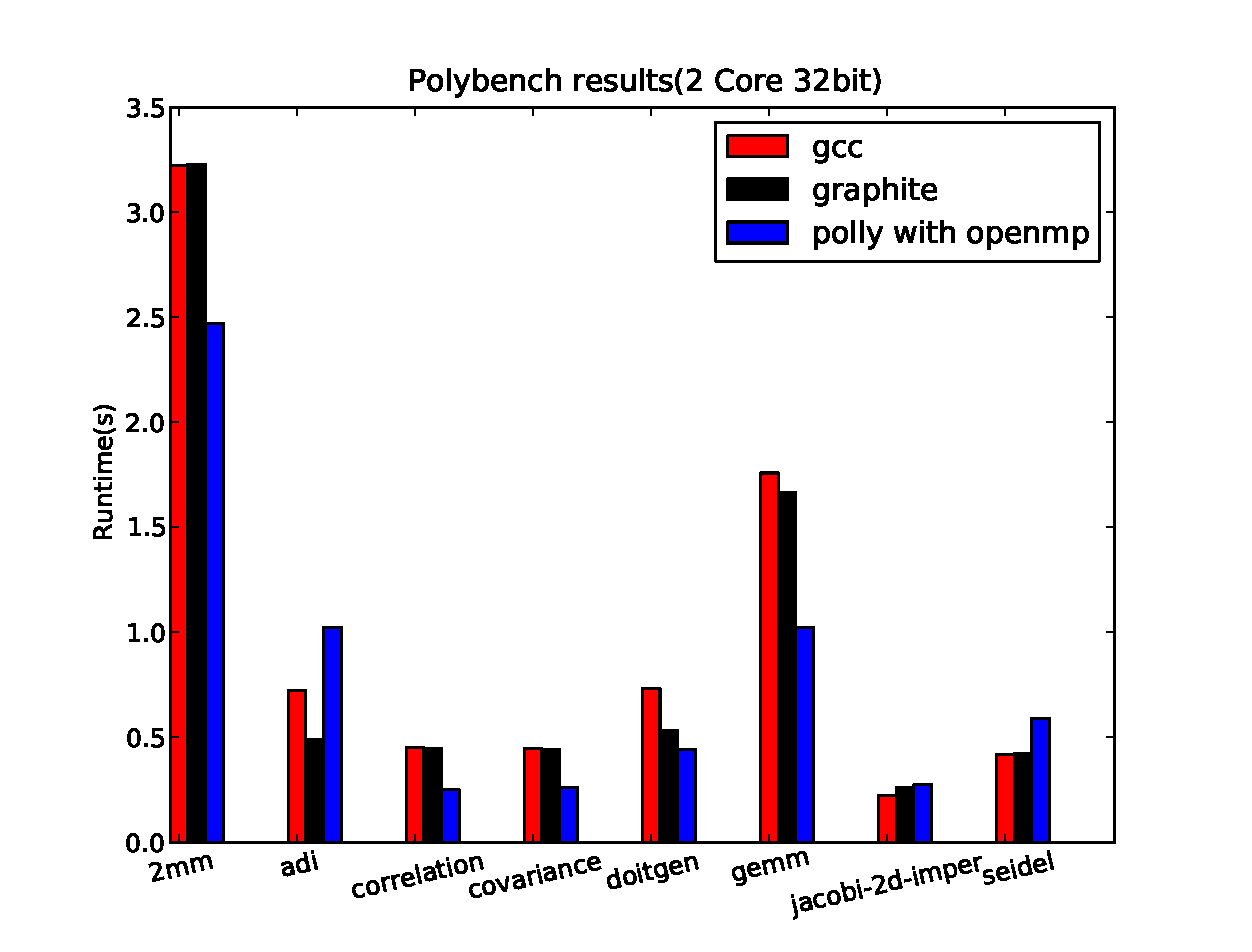
\includegraphics[width=1\textwidth]{images/2core32bit.eps}
  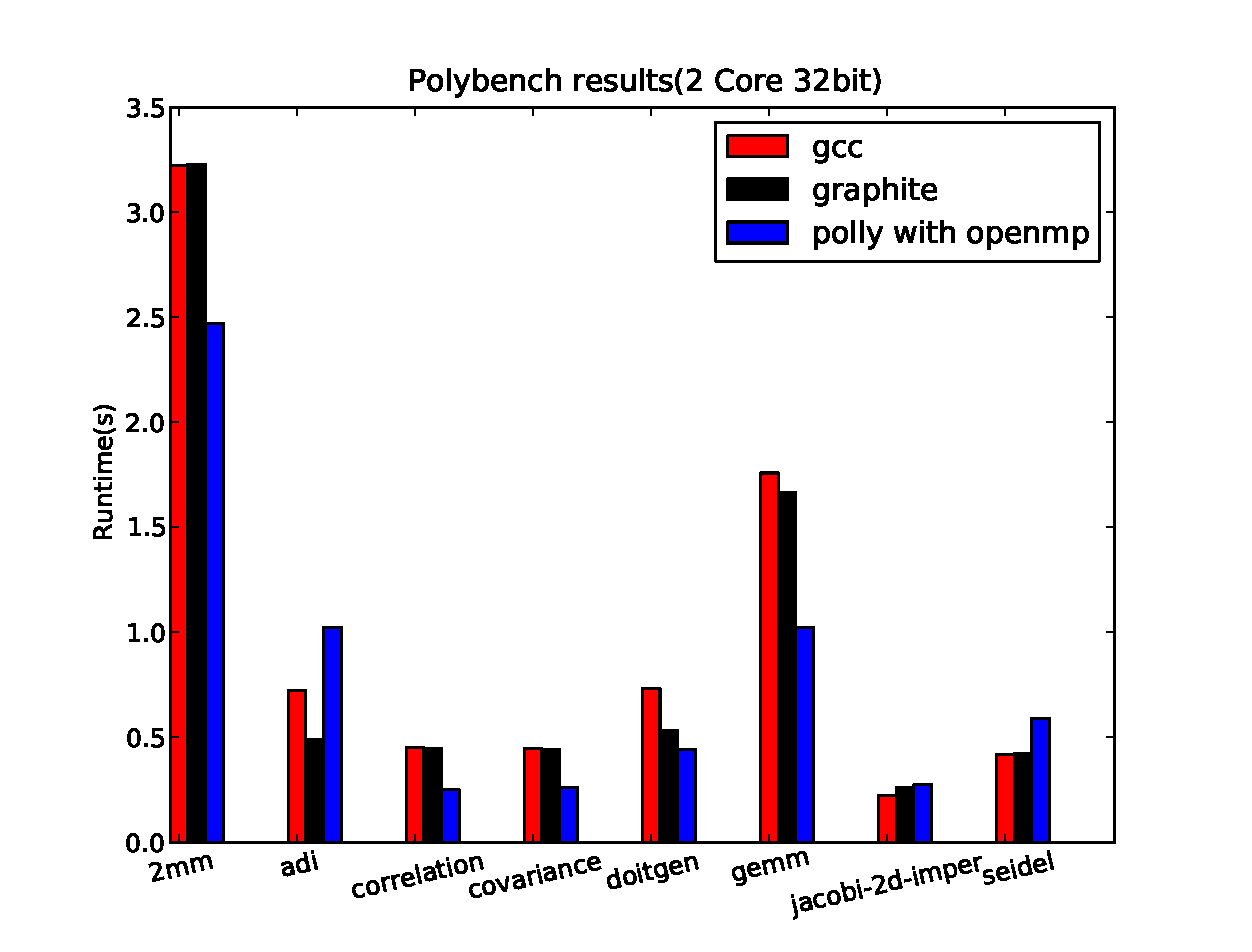
\includegraphics[height=9cm]{images/2core32bit.eps}
  \caption{Performance comparison(2 core 32 bit)}
  \label{fig:2core1}
\end{center}
\end{figure}

\begin{figure}
\begin{center}
  %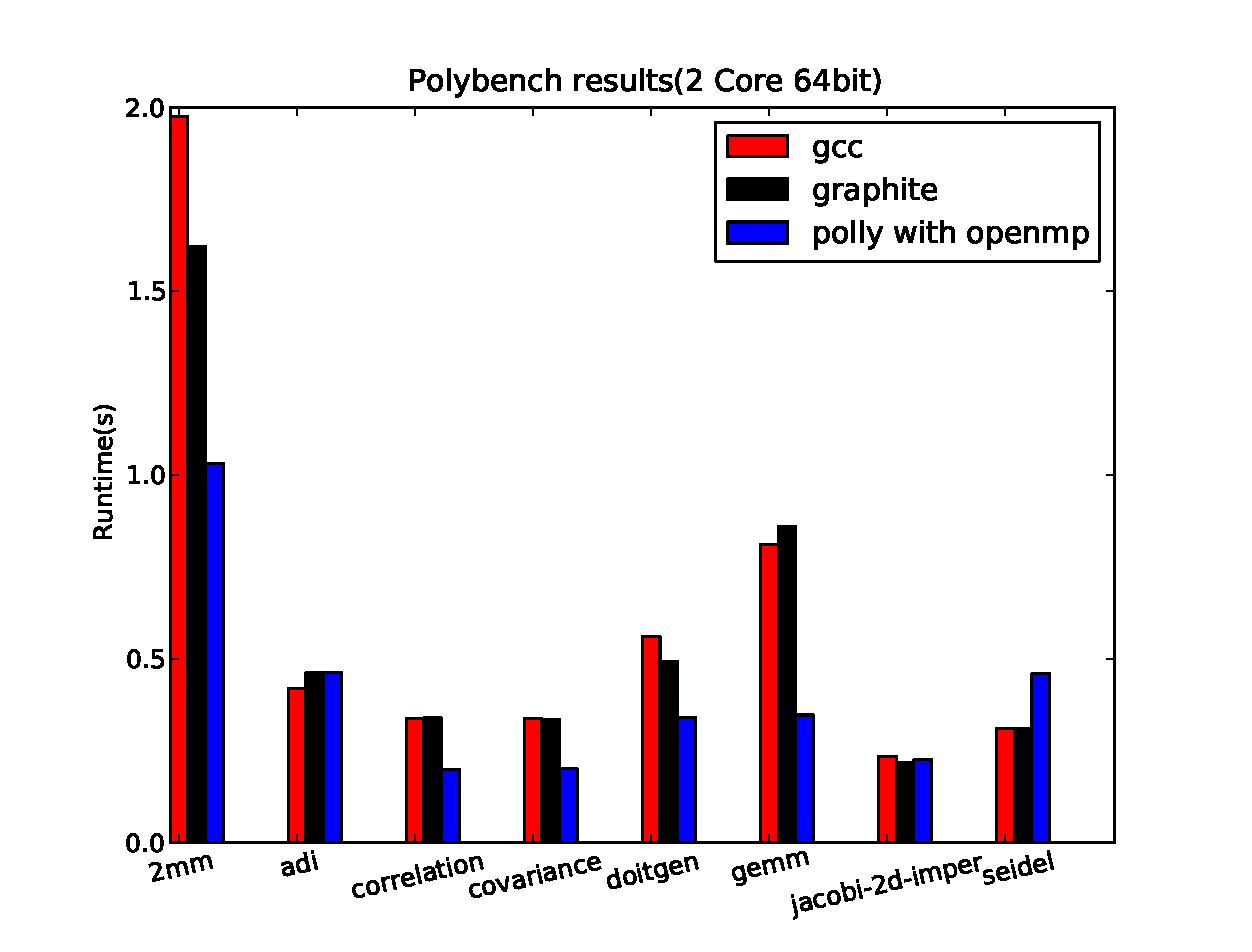
\includegraphics[width=1\textwidth]{images/2core64bit.eps}
  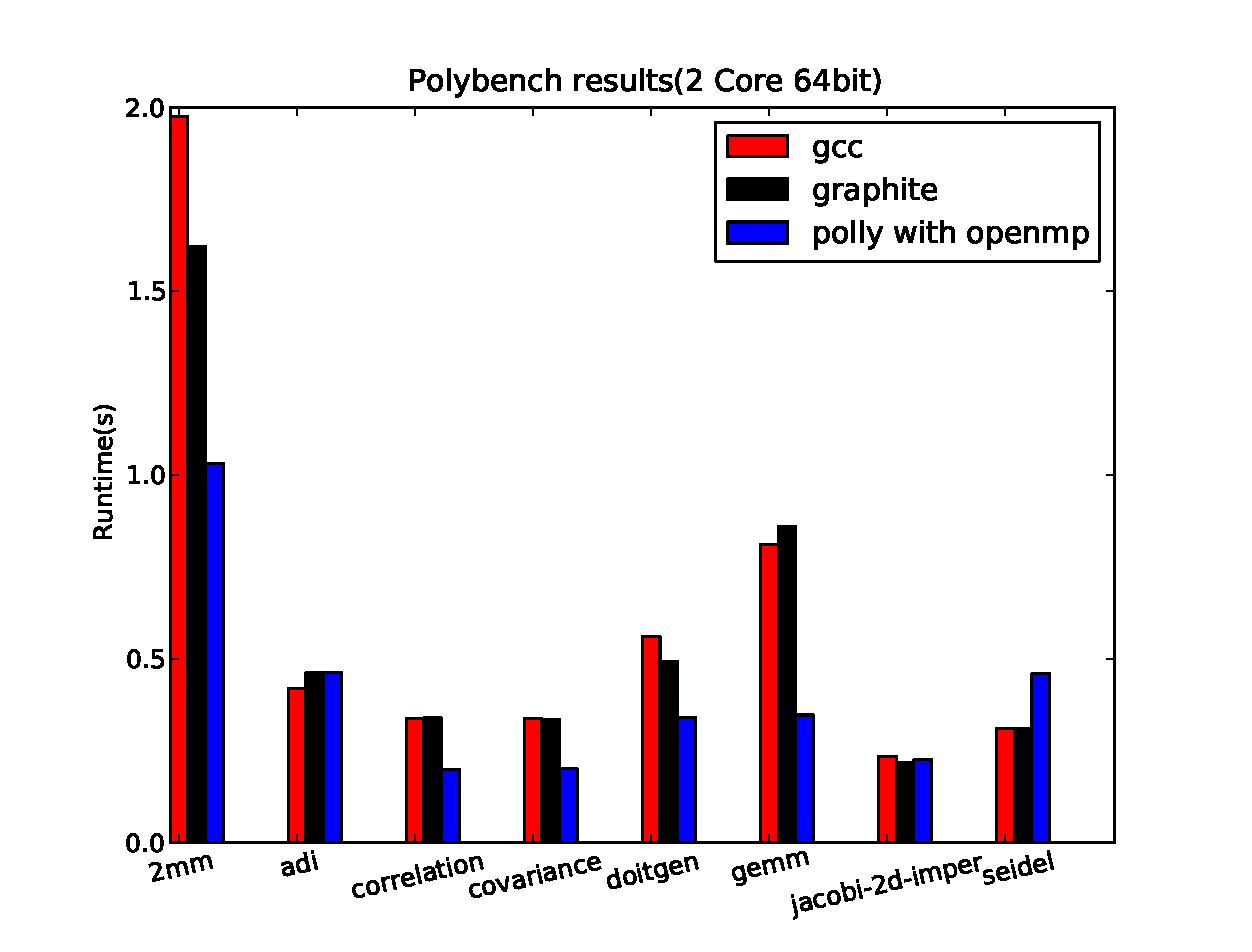
\includegraphics[height=9cm]{images/2core64bit.eps}
  \caption{Performance comparison(2 core 64bit)}
  \label{fig:2core2}
\end{center}
\end{figure}

\begin{figure}
\begin{center}
  %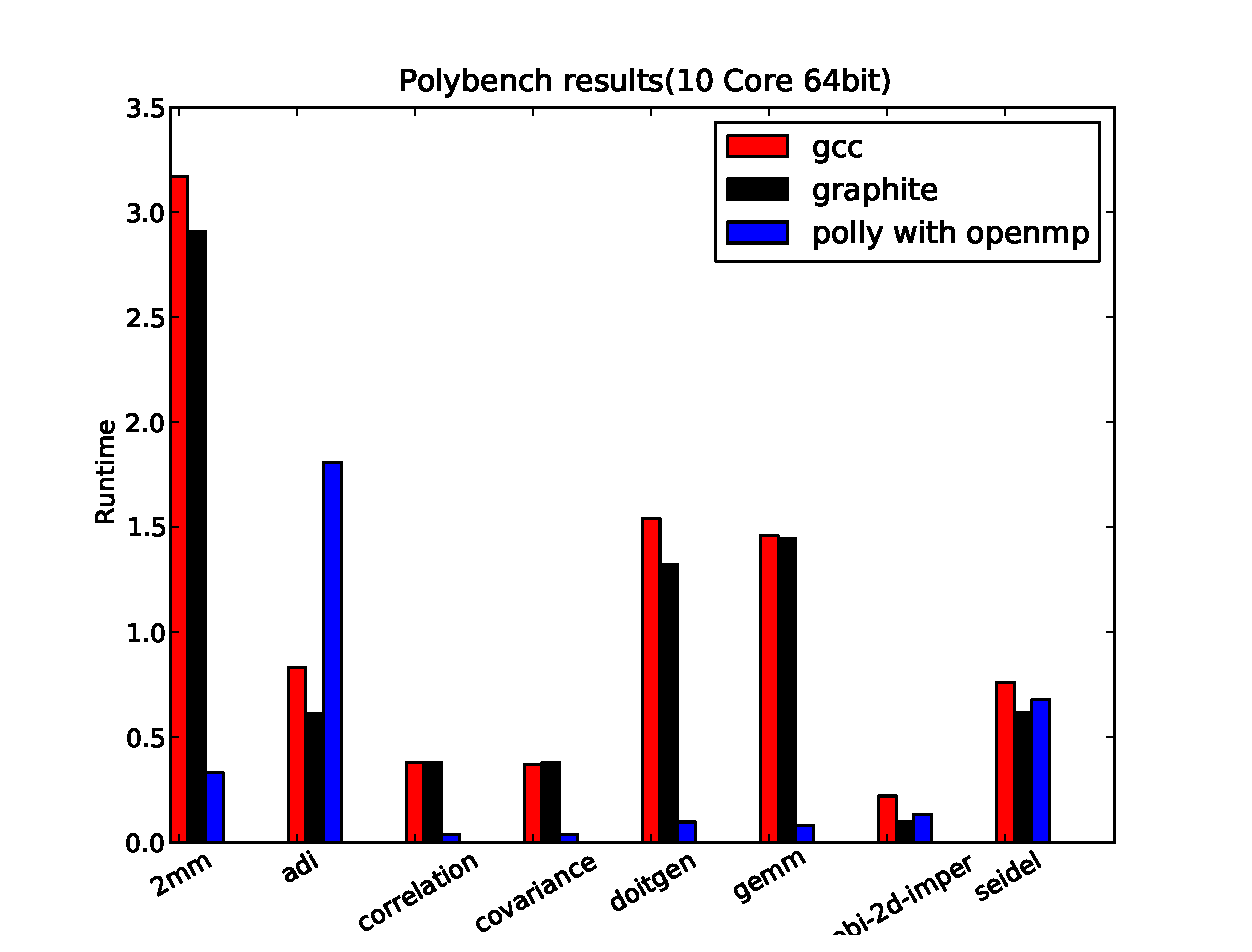
\includegraphics[width=1\textwidth]{images/10core64bit.eps}
  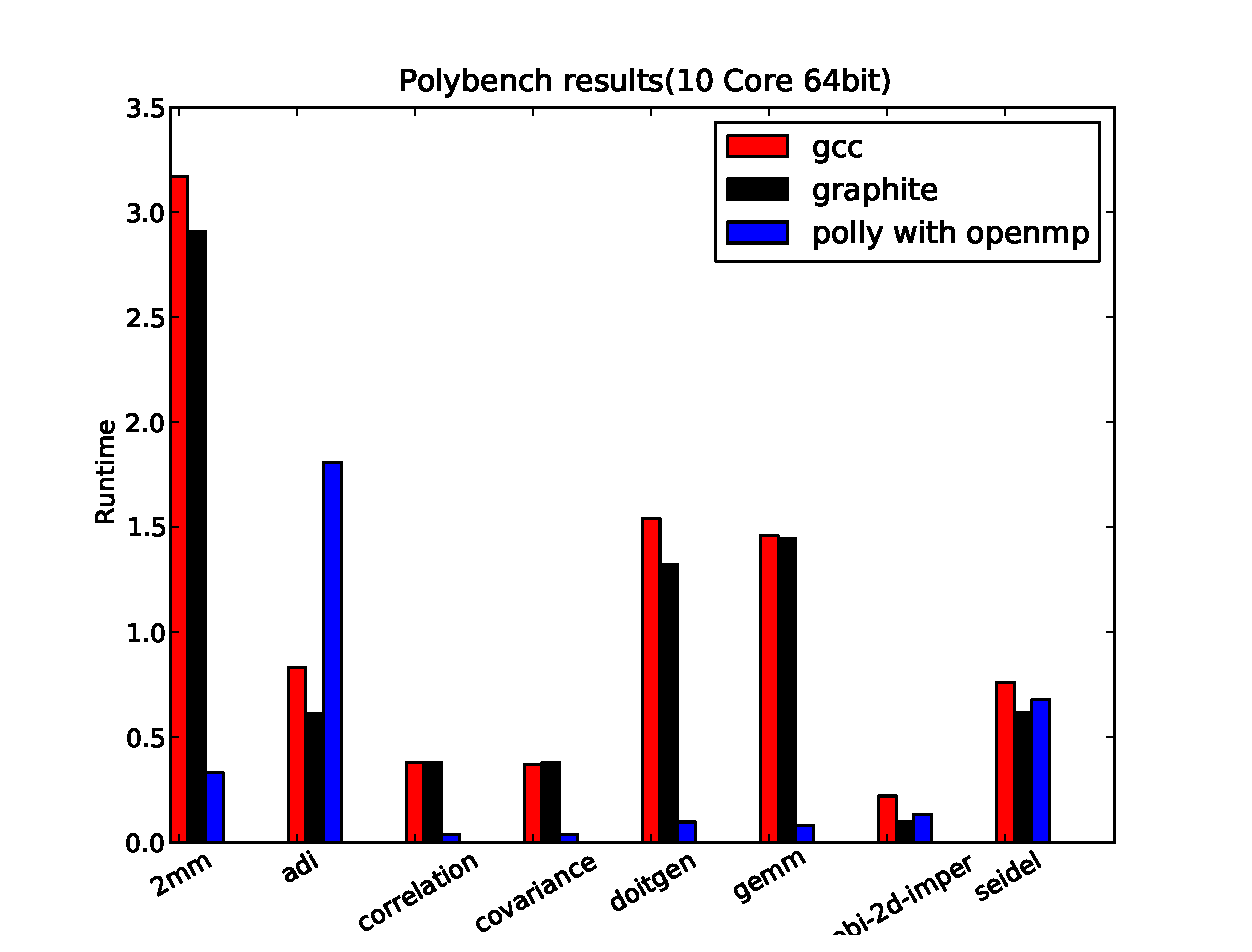
\includegraphics[height=9cm]{images/10core64bit.eps}
  \caption{Performance comparison(10-core 64 bit)}
  \label{fig:10core}
\end{center}
\end{figure}

The OpenMP code generated by Polly is compared with gcc and graphite\cite{TRIFUNOVIC:2010}. With gcc
we make a comparison with serial execution and with graphite we make comparison
with an existing autoparallelization framework, which is also based on polyhedral
model. 
The tests are carried out in 3 different machine with the following configurations

\begin{itemize}
\item Intel Core 2 Duo with 32 Bit OS
\item Intel Core 2 Duo with 64 bit OS
\item 10-Core AMD Engineering Sample with 64 Bit OS
\end{itemize}
The 10-core machine is part of GCC compile farm\footnote{\url{http://gcc.gnu.org/wiki/CompileFarm}}. The GCC Compile farm project maintains
a set of machines of various architectures and provides ssh access to free software developers, GCC and others.
Once the account application  is approved, we get full ssh access to all the farm machines. Then we
are free to install any packages and test our work. The only prerequisite to get access is that
we should be an active contributer for at least one free software project.

The script for testing is given below and the results are shown in the graphs in
Figures ~\ref{fig:2core1}, ~\ref{fig:2core2} and ~\ref{fig:10core}.
{\footnotesize
\begin{lstlisting}
# serial
gcc -I utilities utilities/instrument.c -DPOLYBENCH_TIME   \
                      -DPOLYBENCH_DUMP_ARRAYS -O3 $1 -lm
# Autopar with graphite
n = 4 # n = 2 for 2 core, n = 10 for 10-core
gcc -I utilities utilities/instrument.c -DPOLYBENCH_TIME   \
           -DPOLYBENCH_DUMP_ARRAYS -O3 -floop-interchange  \
           -floop-block -floop-parallelize-all             \
	   -ftree-parallelize-loops=$n $1 -lm
# Autopar with polly OpenMP
pollycc -fpolly -fparallel -I utilities utilities/instrument.c \
              -DPOLYBENCH_TIME -DPOLYBENCH_DUMP_ARRAYS  $1 -lm
\end{lstlisting}
}
While we look into the results it can be observed that Polly with OpenMP support
shows nice performance other than the benchmarks 'adi' and 'seidel'. It is observed
that the core loops in these testcases are detected as SCoPs and detected as parallel. OpenMP
code is generated for them too. The reason for the overhead is yet to be investigated and such cases will be part of one
of the future work(Increasing coverage of Polly). For details refer to Chapter ~\ref{chap:future}.



